\documentclass[main.tex]{subfiles} 

\begin{document}
%%%%%%%%%%%%%%%%%%%%%%%%%%%%%%%%%%%%%%%%%%%%%%%%%%%%%
%%%%%%%%%%%%%%%%    Appendices   %%%%%%%%%%%%%%%%%%%%
%%%%%%%%%%%%%%%%%%%%%%%%%%%%%%%%%%%%%%%%%%%%%%%%%%%%%
\appendix
\section{Klassebeskrivelse}
Skolen er lokalisert i et godt sosioøkonomisk område, deriblant har foreldrene til elevene høy
utdanningsbakgrunn. 8.klassen består av 13 gutter og 11 jenter. En skoletime varer i 50
minutter, efterfulgt av en 10 minutter lang pause. Elevene ved skolen har i gjennomsnitt 27.6
timer i uka. I klassen sitter elevene to-og-to sammen ved sine pulter i et rutenett. Hver andre
uke byttes plasseringene til elevene. Elevene blir fordelt sammen med det skolen kaller
læringspartnere. Læreren printer et nytt klassekart som han/hun har tilgjengelig på sin
kateter/podium. Elever pleier å legge fra sine mobiler i en hylleplass eller deres bokskap. Når en
time starter, står elevene opp i sine stoler og hilser på læreren før de får lov til sitte. Tavlen
brukes sjelden, siden lystavlen er ofte plassert i alle klasserom foran tavlen. Onenote brukes
flittig gjennom undervisning og til planleggingen av undervisningen. Elevene har også blitt
velkjent med Onenote ved å se lærere bruke den, og selv bruke den i sine delingstimer. Lekser
blir ført i It’s Learning plattformen. I klassen vi observerte kommer det 3 elever fra
velkomstklassen som deltar i undervisning torsdag og fredag hver uke. Disse elevene har ofte
problemmer med å forstå norsk, men de er flinkere til å lese og skrive. I blant bruker deres
kontaktlærer engelsk for å formidle informasjon. Men som regel blir helklasse undervisningen
ført i norsk. Det er generelt ingen sosiale problemmer eller konflikter i klassen, og elevene pleier
å samarbeide med hverandre uten store problemmer. Skolen har en del problemmer med
elever som trenger en eller annen form for tilrettelegging. I trinnmøter til 8.trinn blir det i blant tatt
opp spørsmål om hvem som skal ha tilpasning og hvordan det skal utføres. Fokuset til skolen er
å tilby sine elever et godt psykososial læringsmiljø.

\newpage\null
%\newgeometry{includefoot,left=2cm,right=2cm,bottom=1cm,top=0cm}
\section{Plan for undervisningsopplegg}
\label{sec:plan}
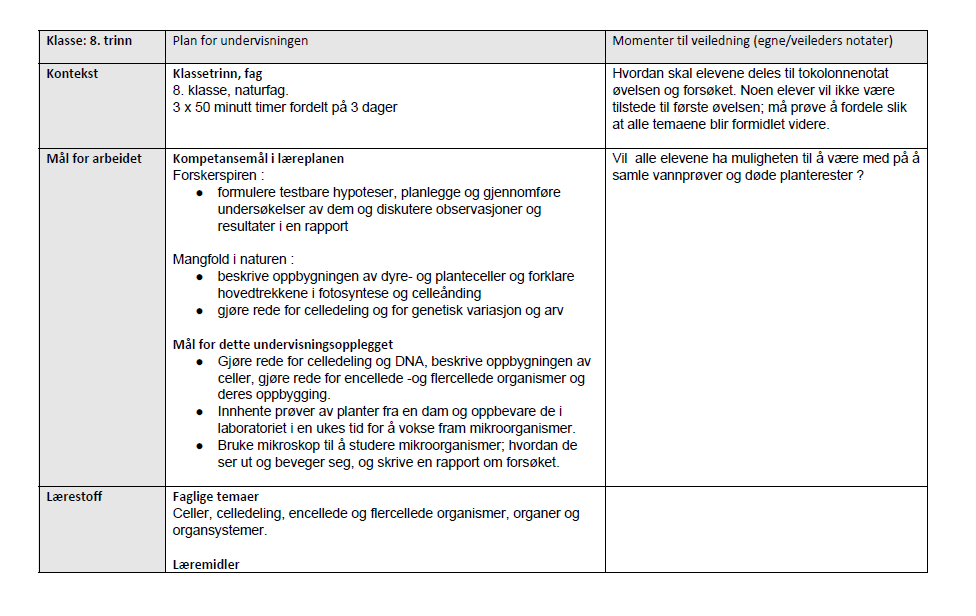
\includegraphics[scale = 0.80,angle=90]{../figures/plan_side1.png}

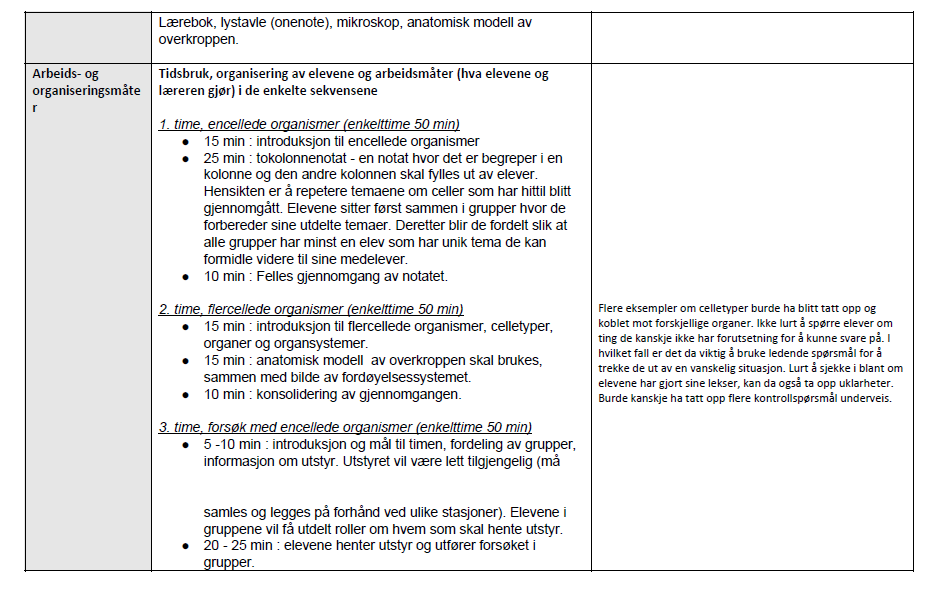
\includegraphics[scale = 0.80,angle=90]{../figures/plan_side2.png}

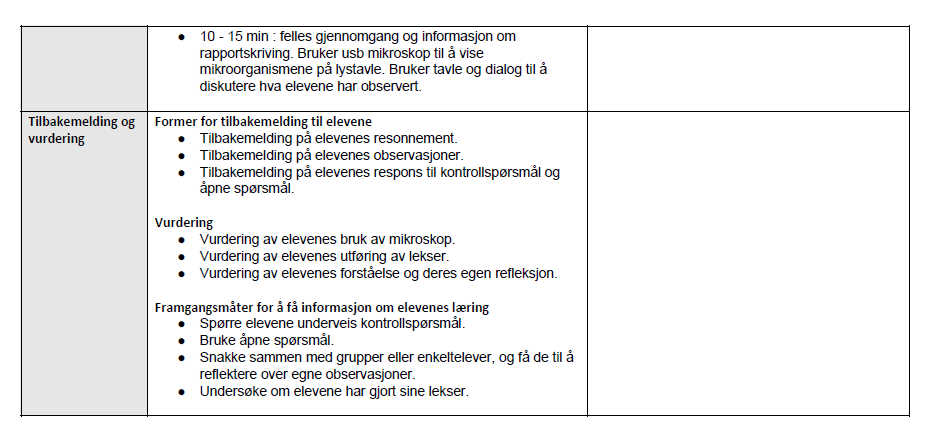
\includegraphics[scale = 0.80,angle=90]{../figures/plan_side3.png}

%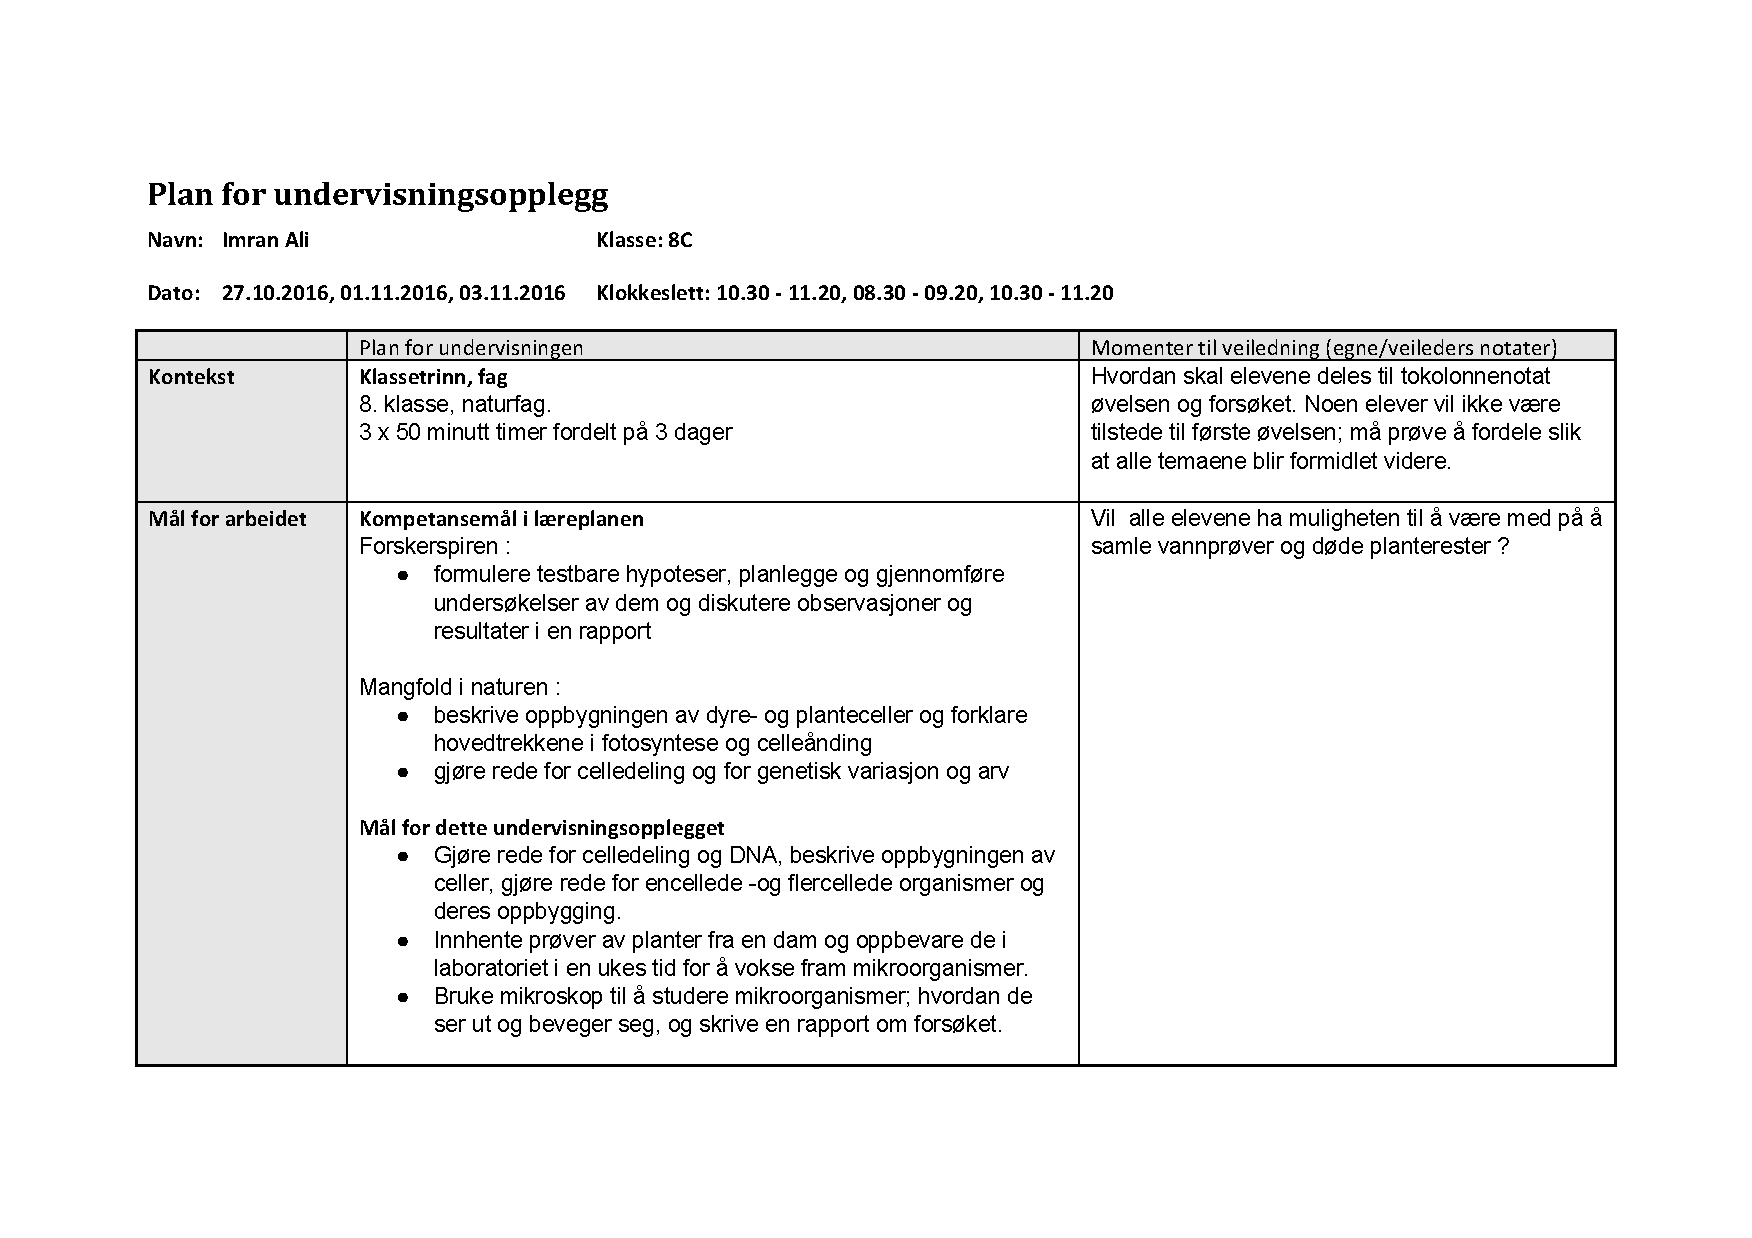
\includepdf[page = 1,scale = 0.9]{../figures/Del_B_plan_for_undervisningsopplegg.pdf}

%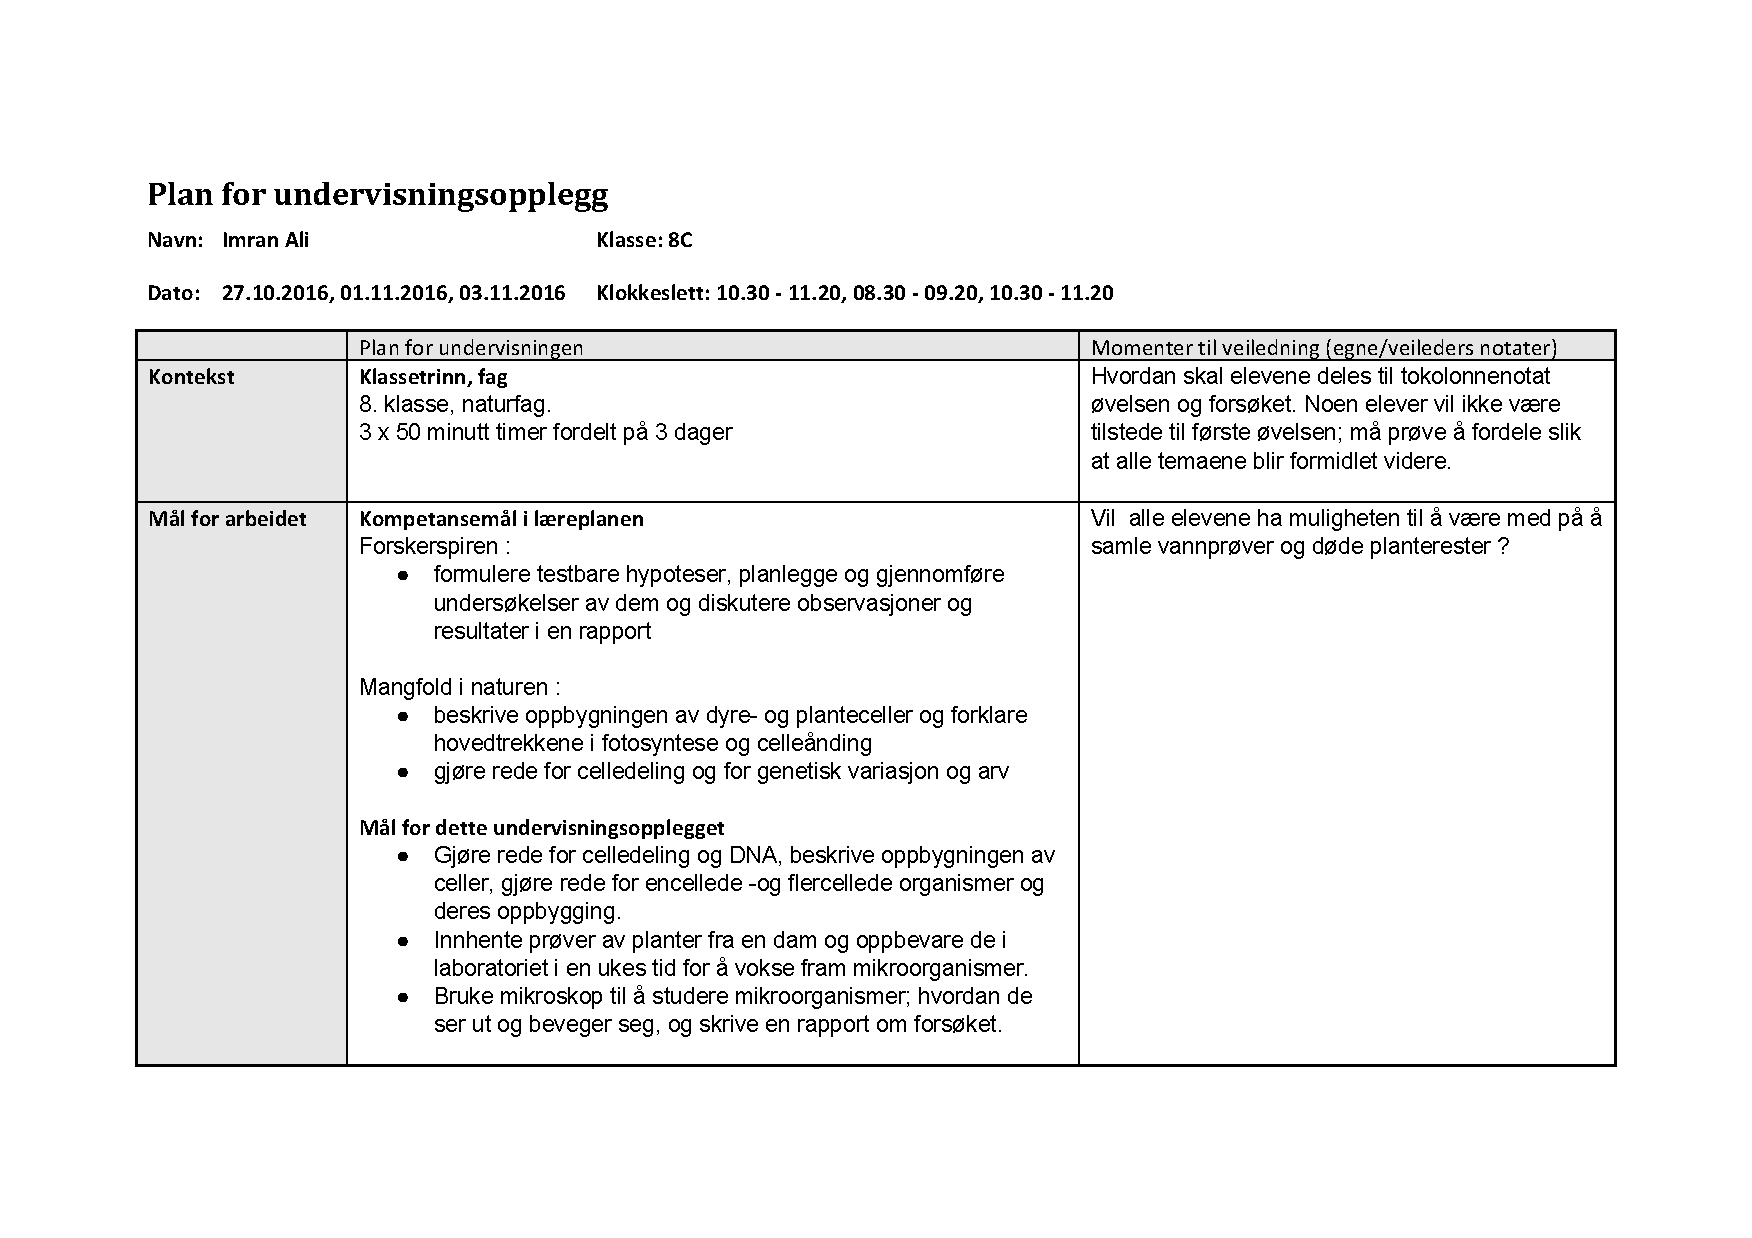
\includepdf[page = 2,scale = 0.9]{../figures/Del_B_plan_for_undervisningsopplegg.pdf}

%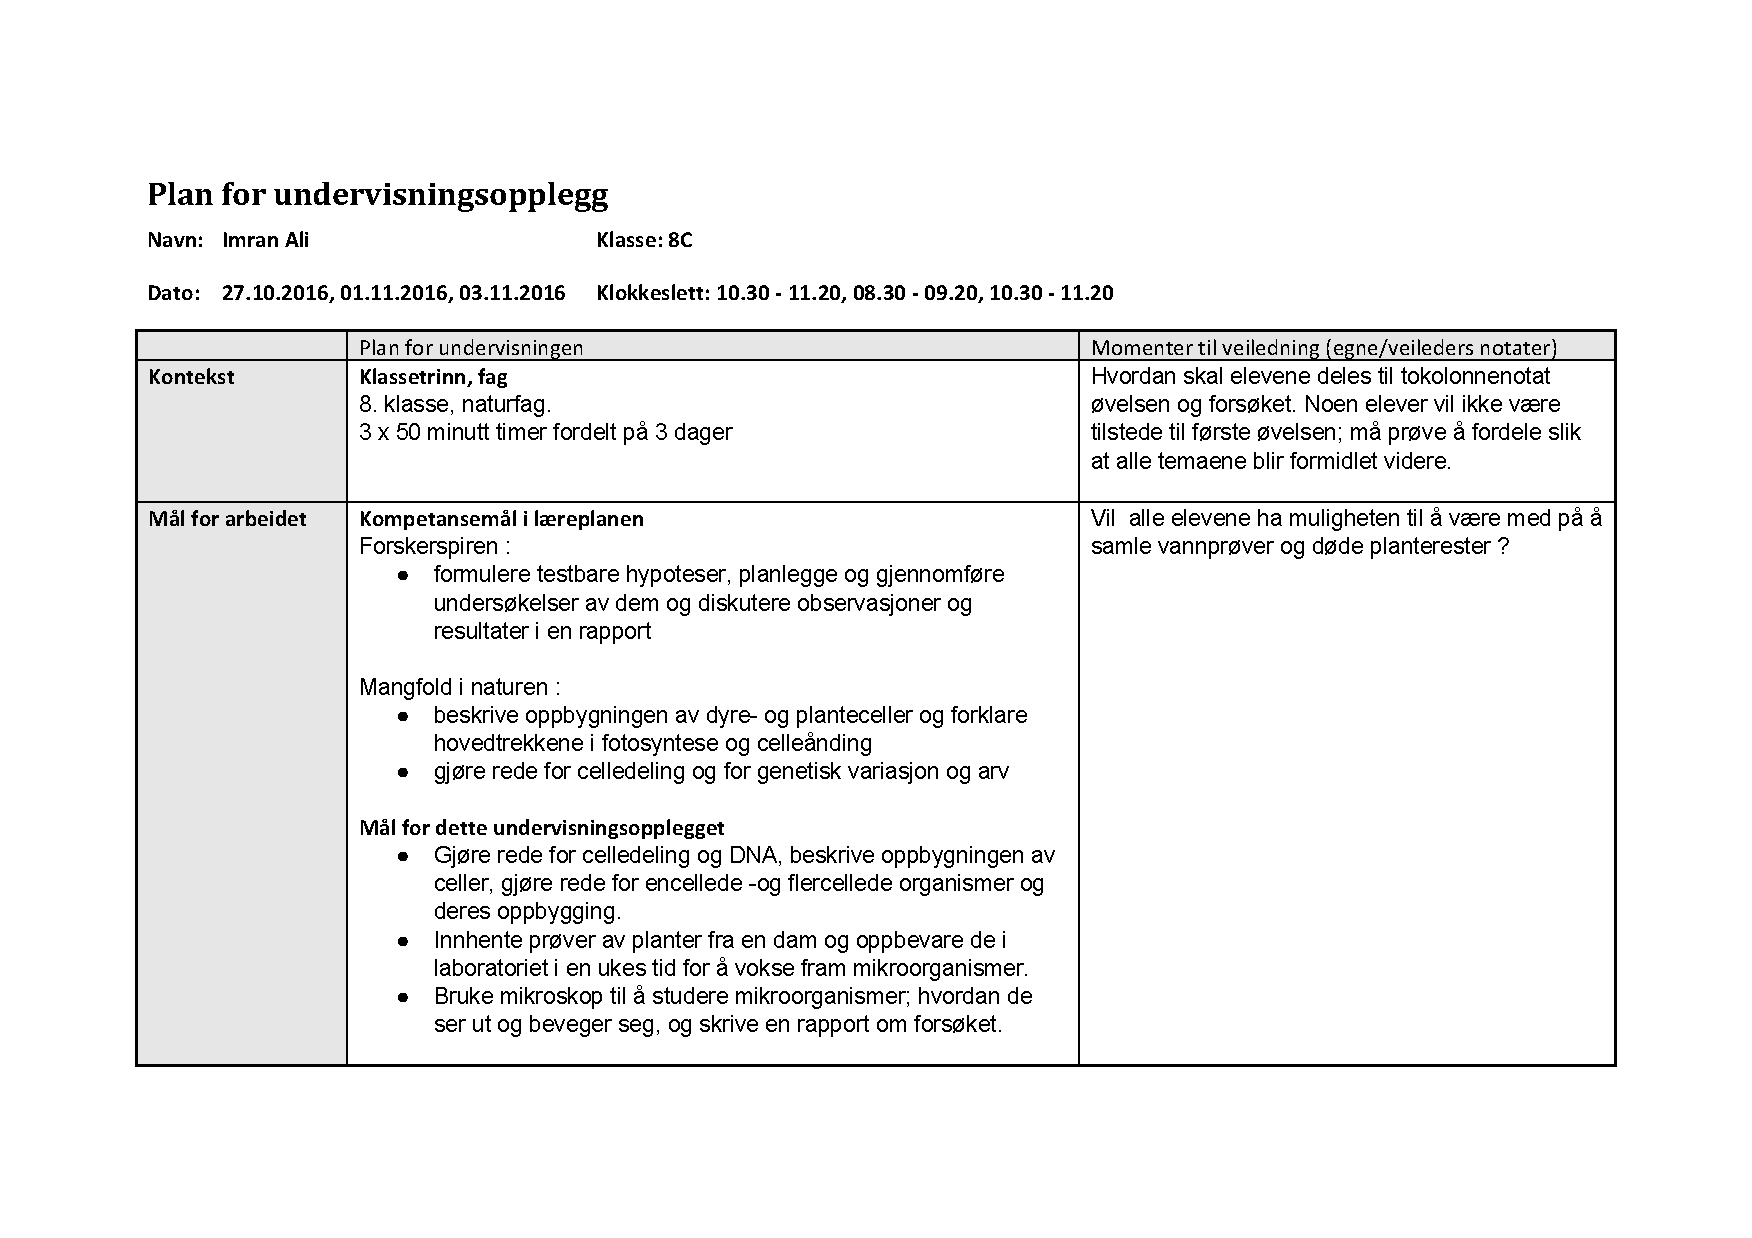
\includepdf[page = 3,scale = 0.9]{../figures/Del_B_plan_for_undervisningsopplegg.pdf}

%\newpage\null
\section{Tokolonnenotat}
\label{sec:tokolonnenotat}
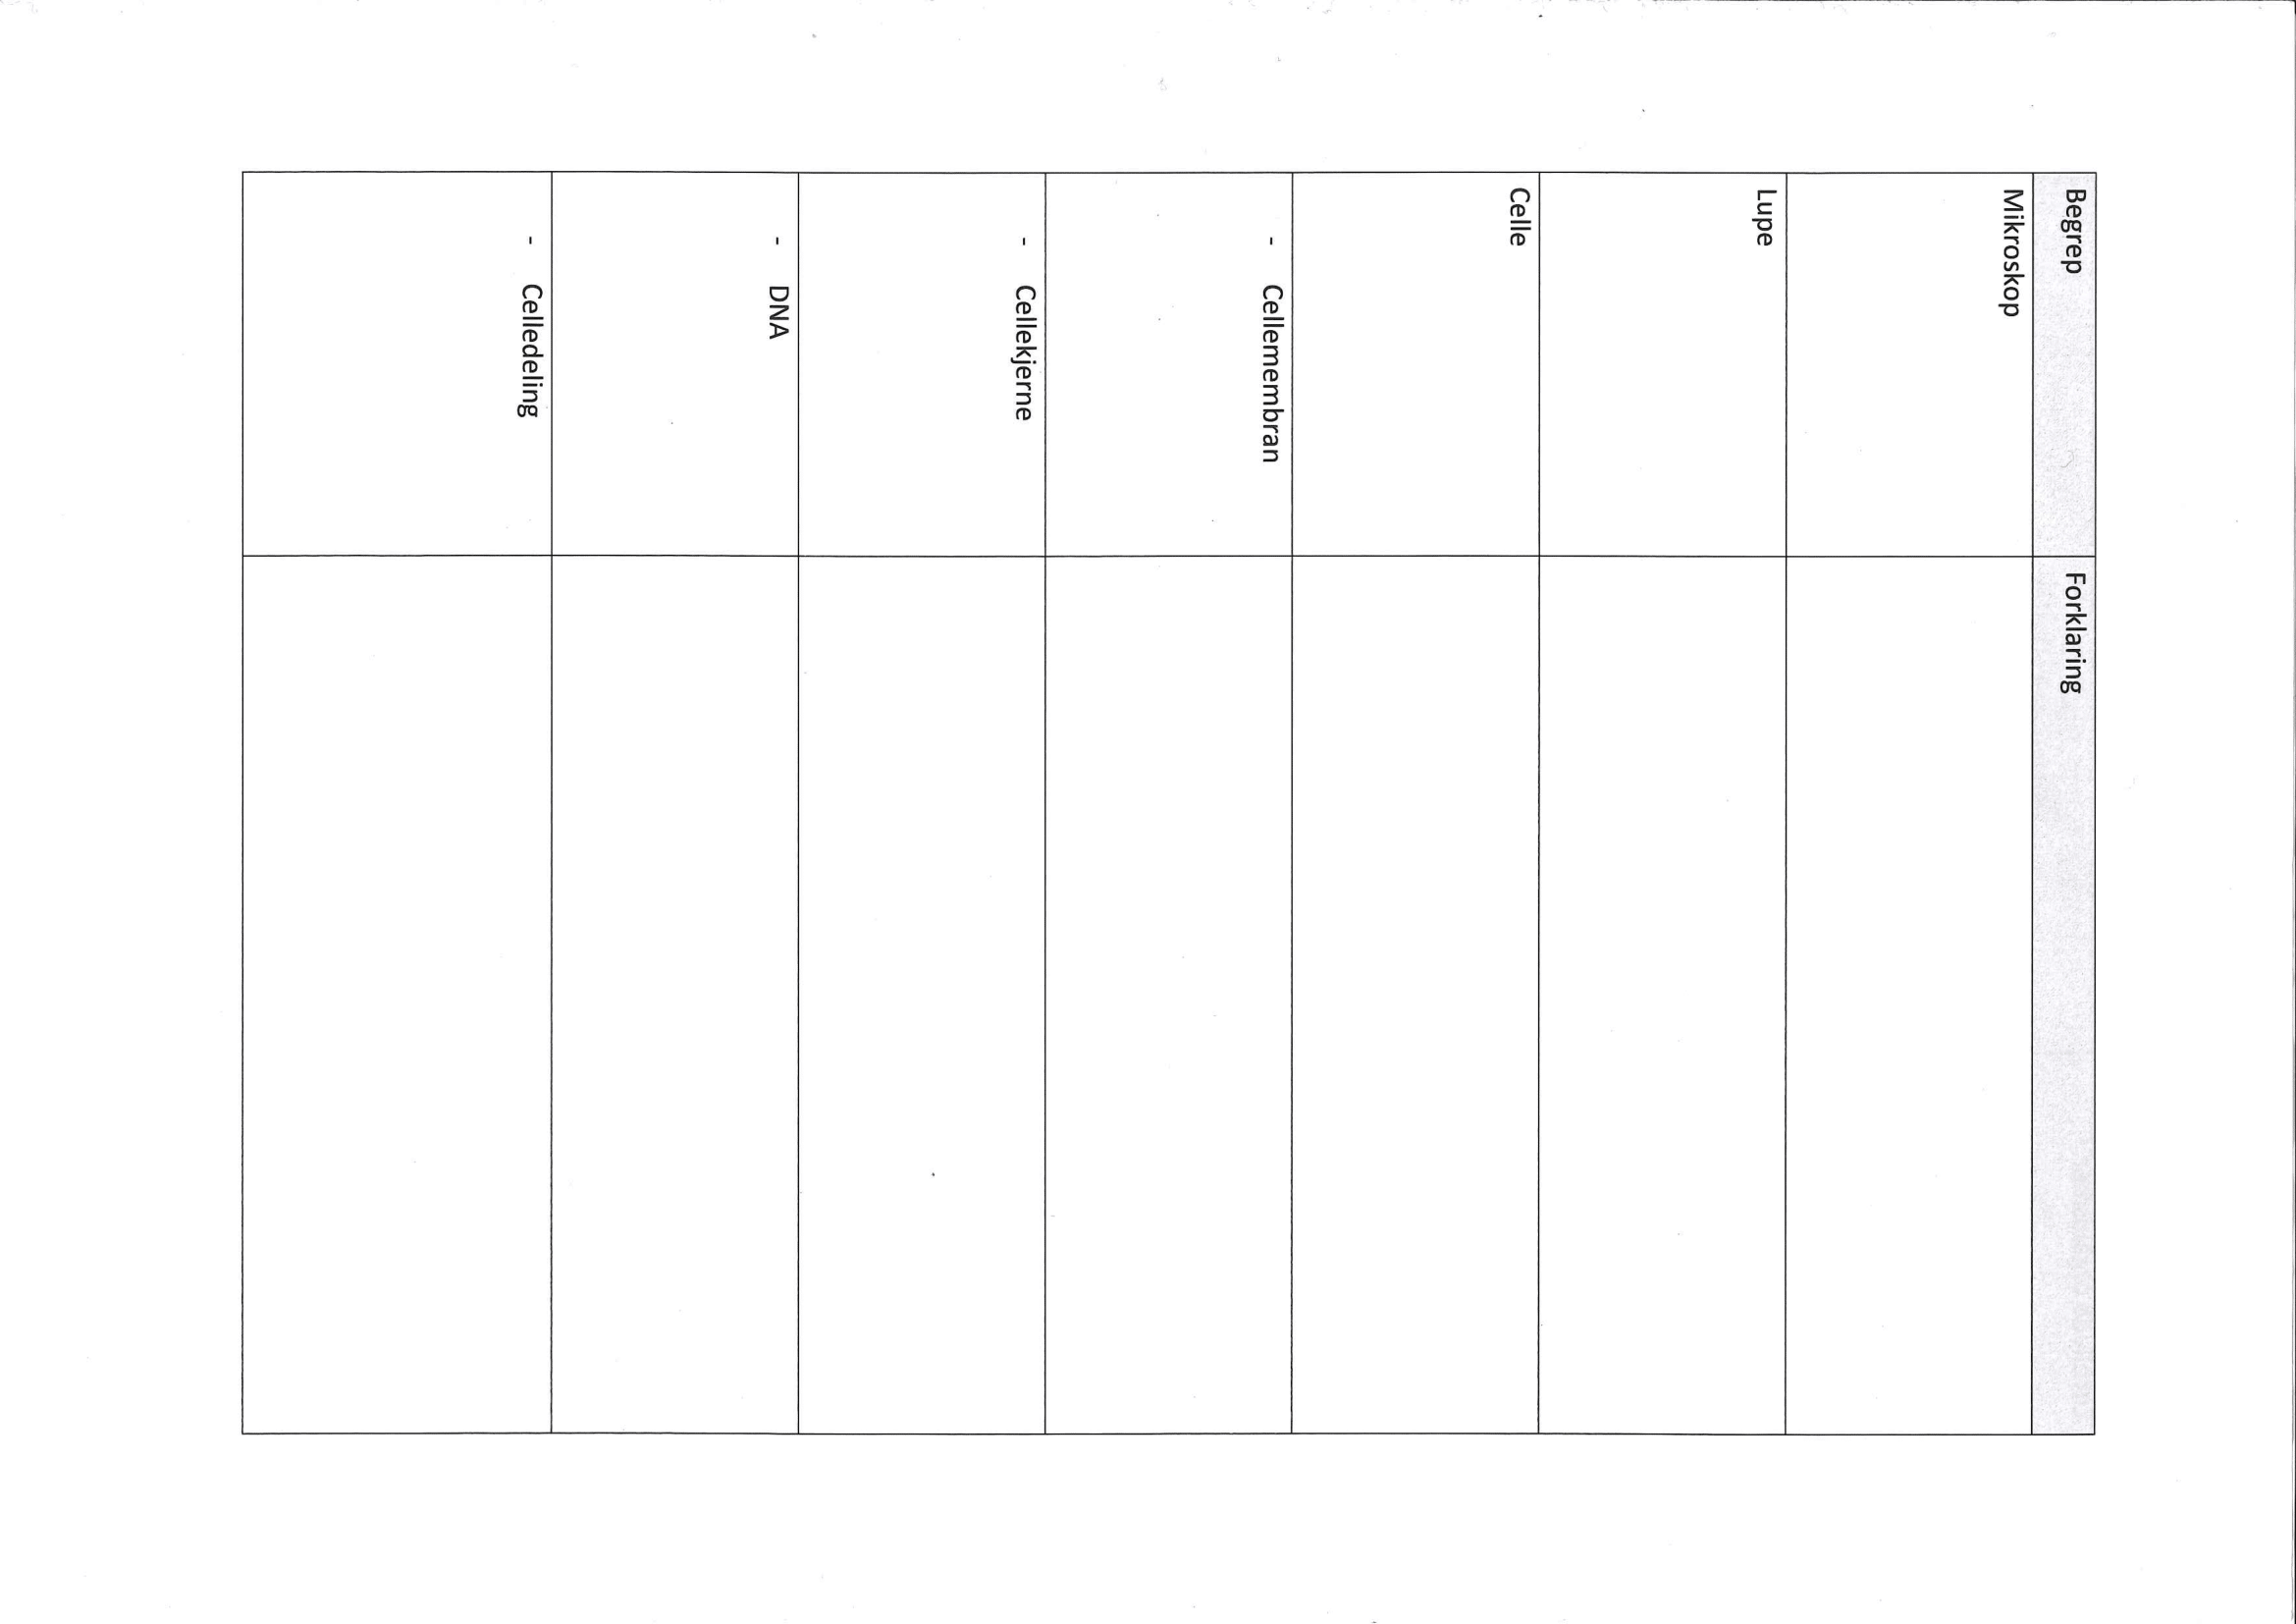
\includegraphics[scale = 0.30,angle=90]{../figures/tokolonnenotat_side1.png}

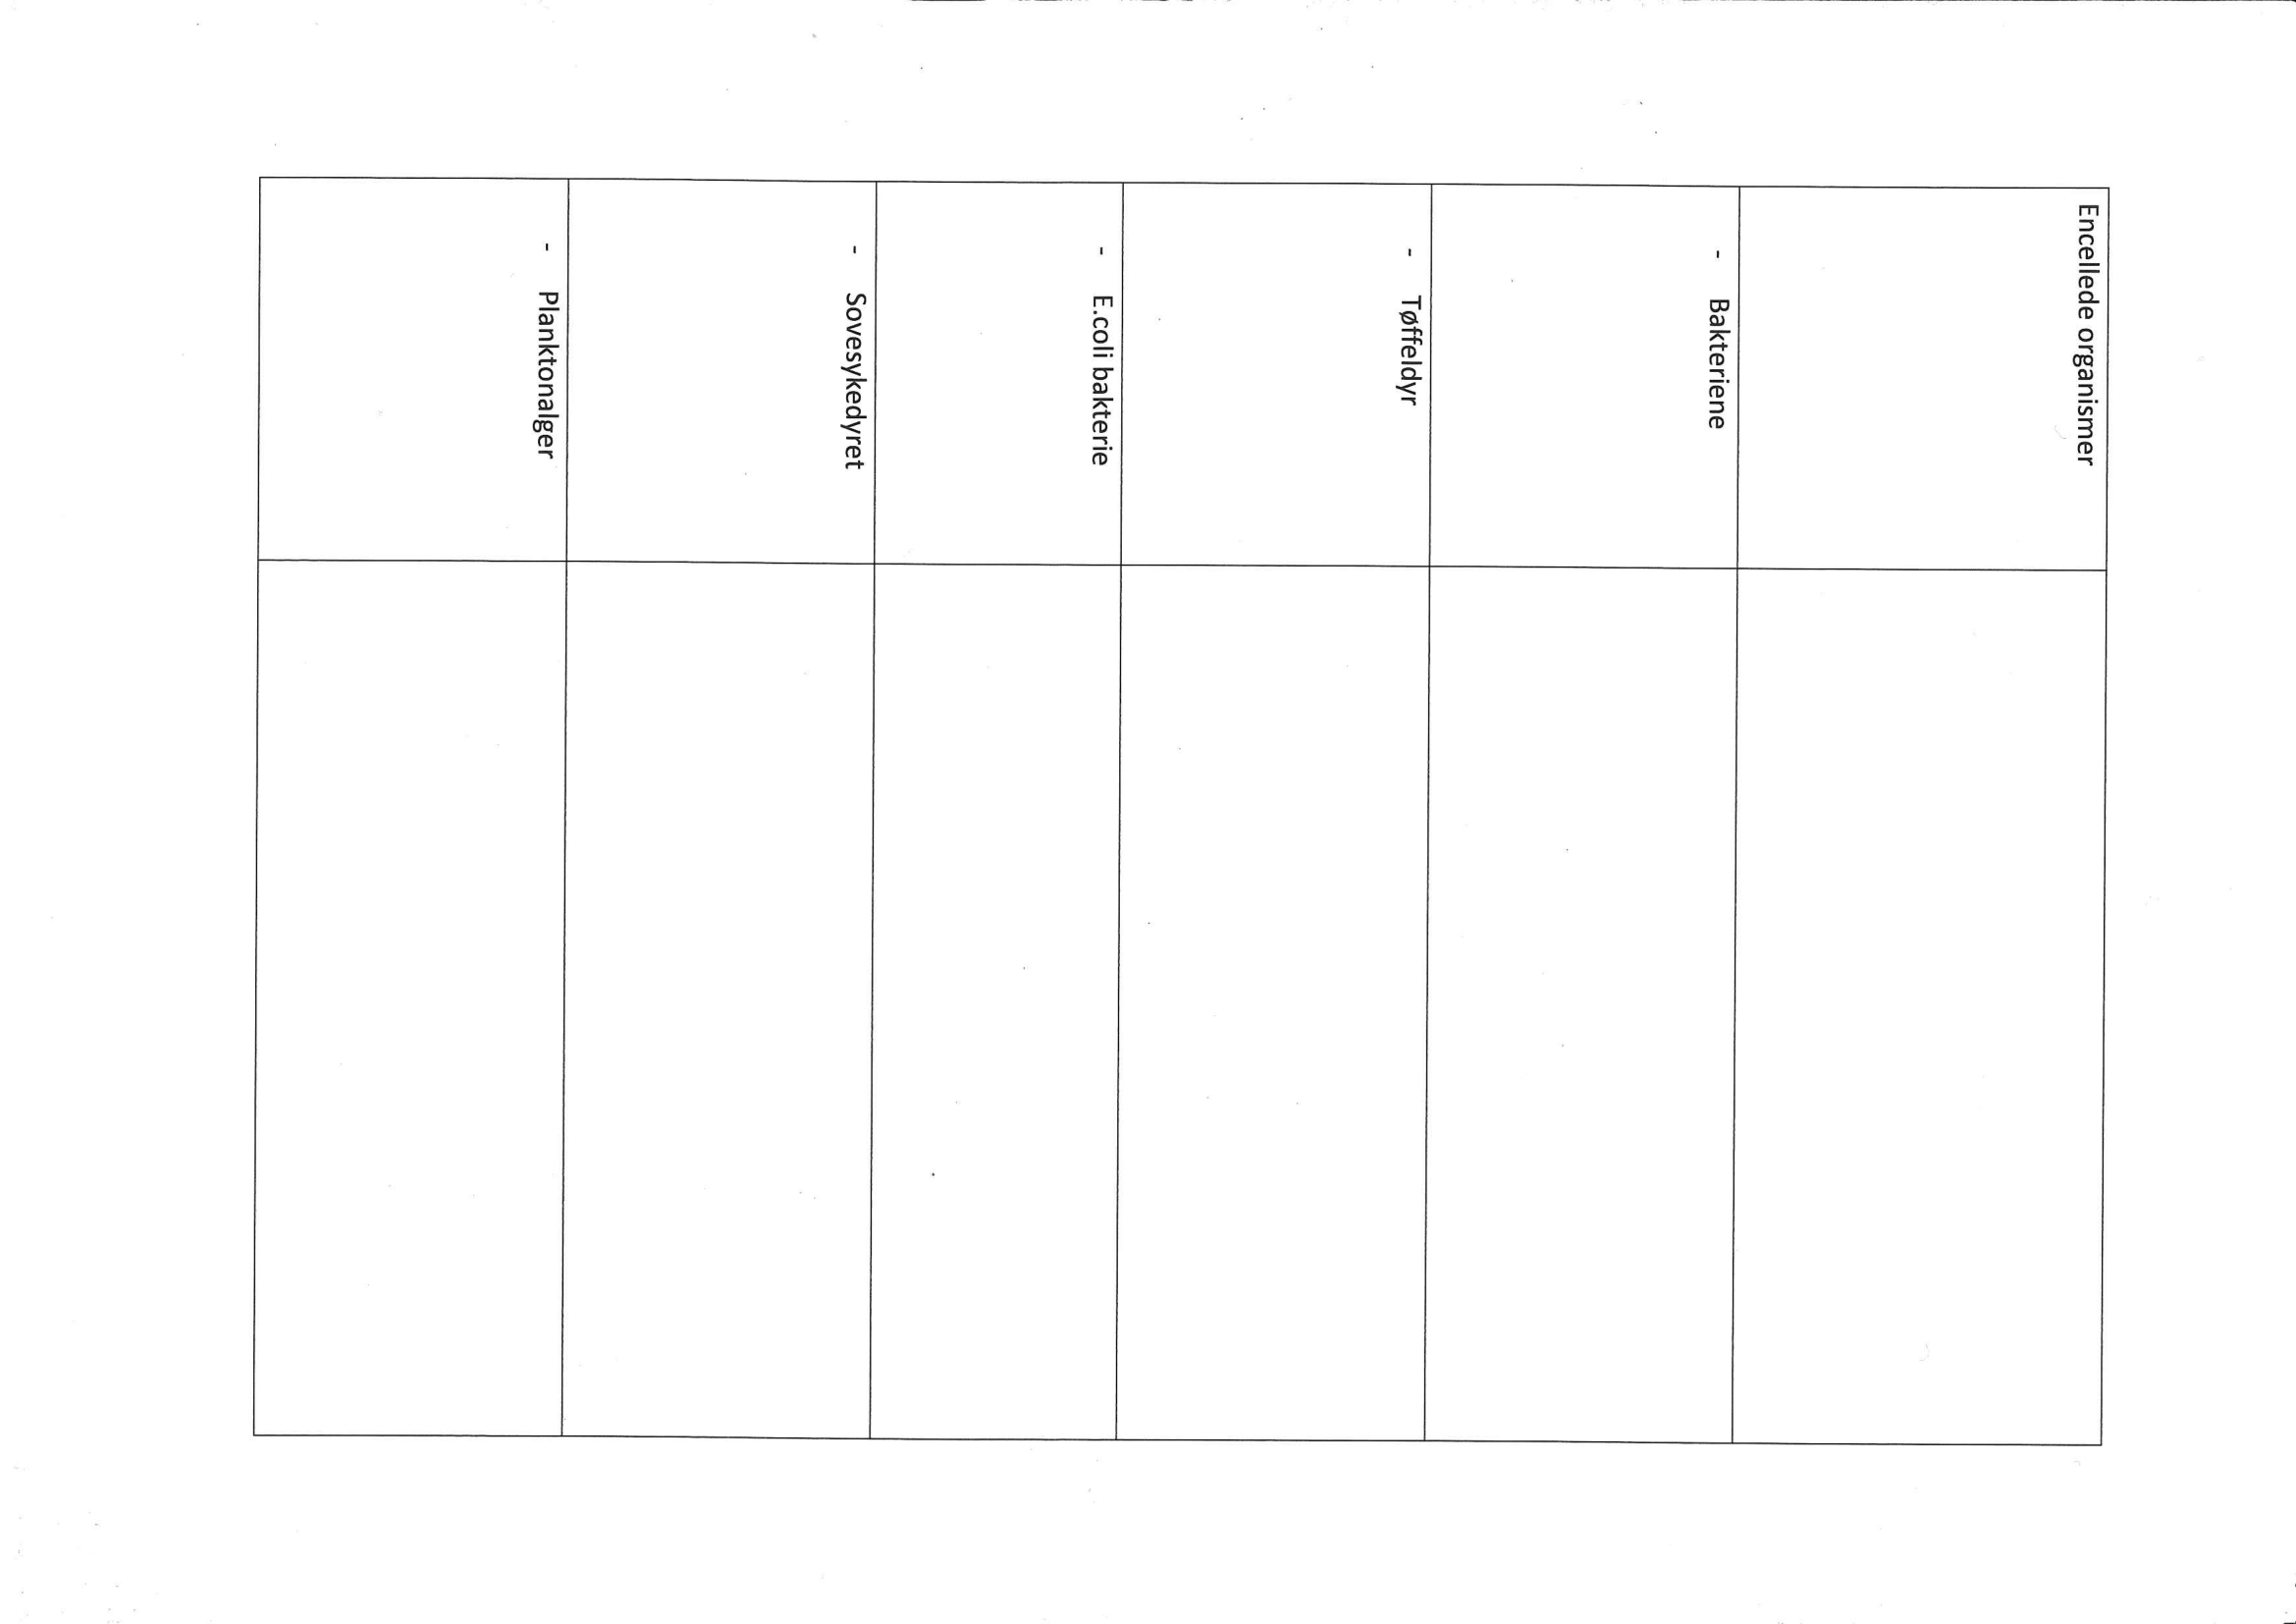
\includegraphics[scale = 0.30,angle=90]{../figures/tokolonnenotat_side2.png}
%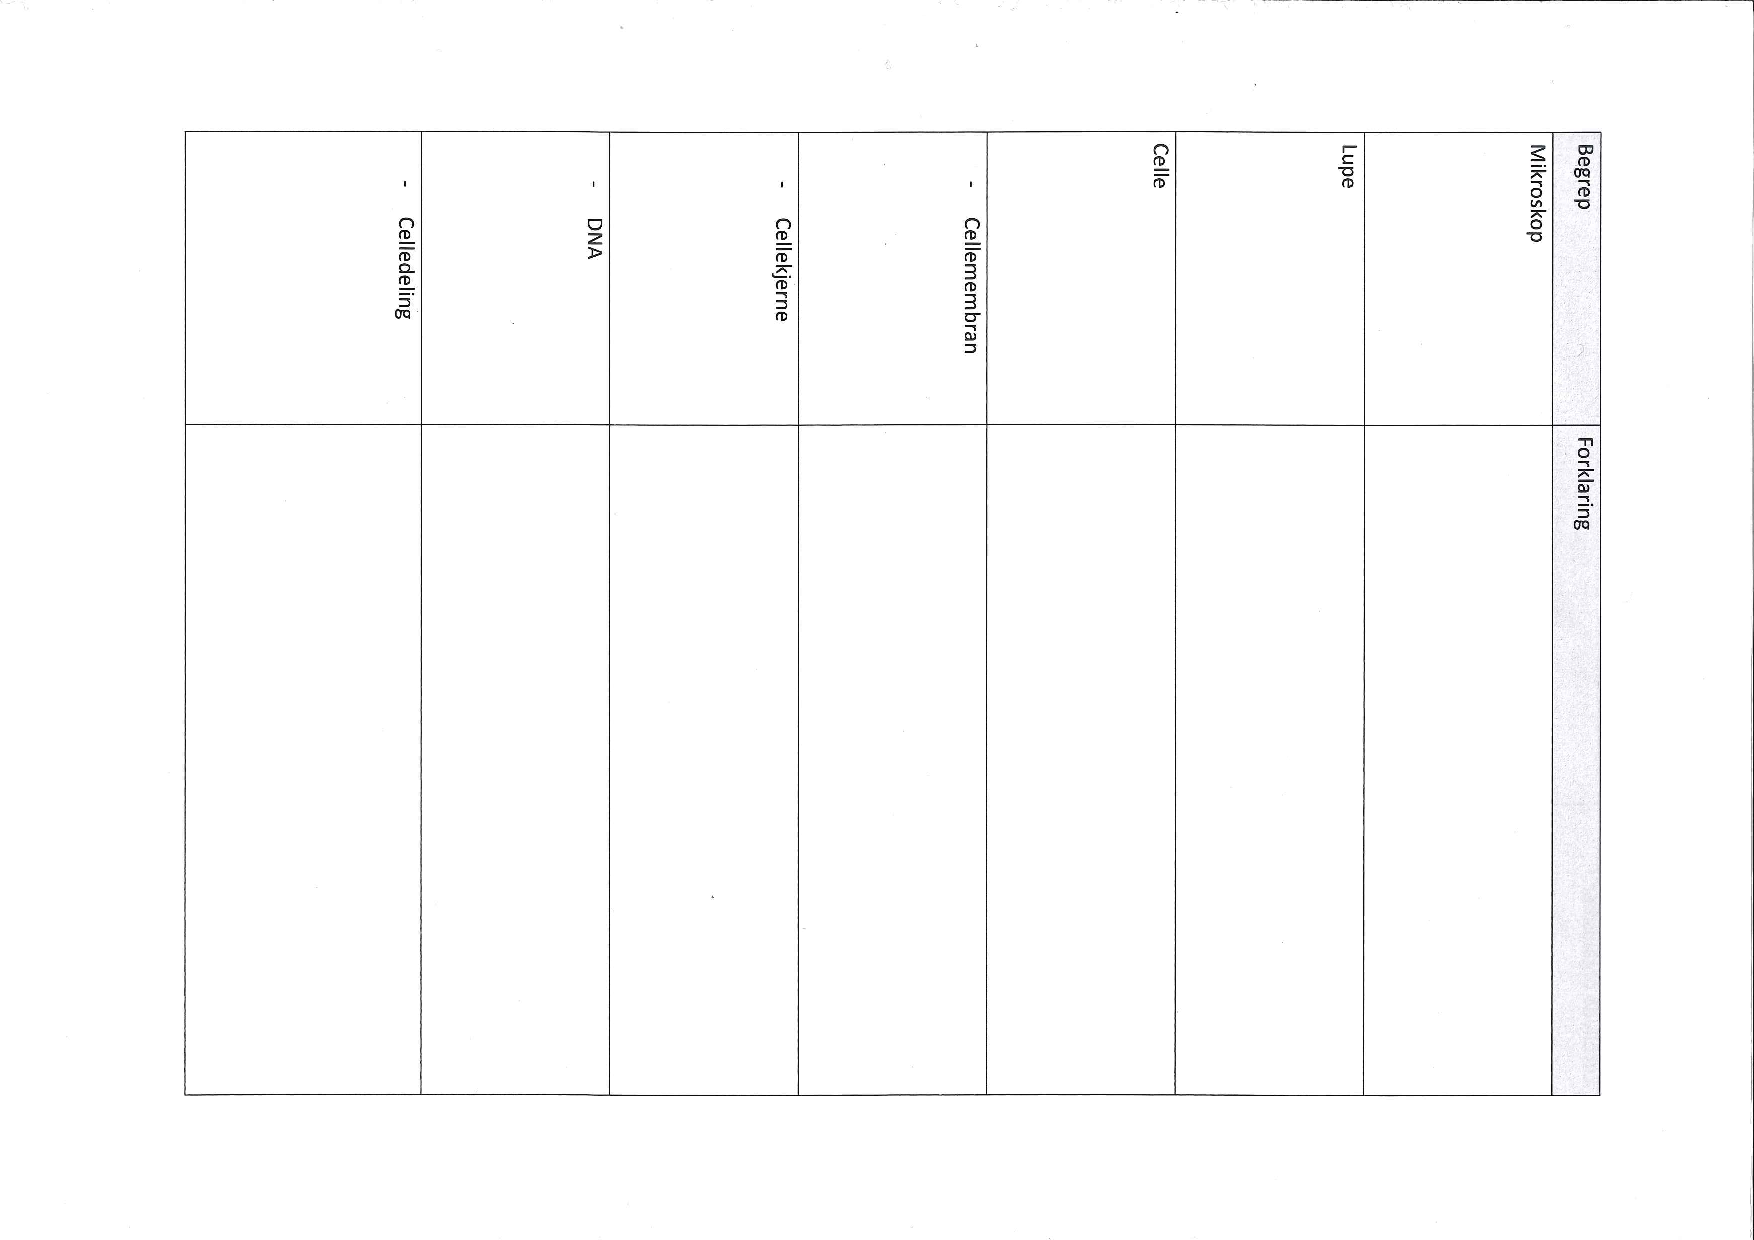
\includepdf[scale = 0.90,angle=90]{../figures/tokolonnenotat_side1.pdf}

%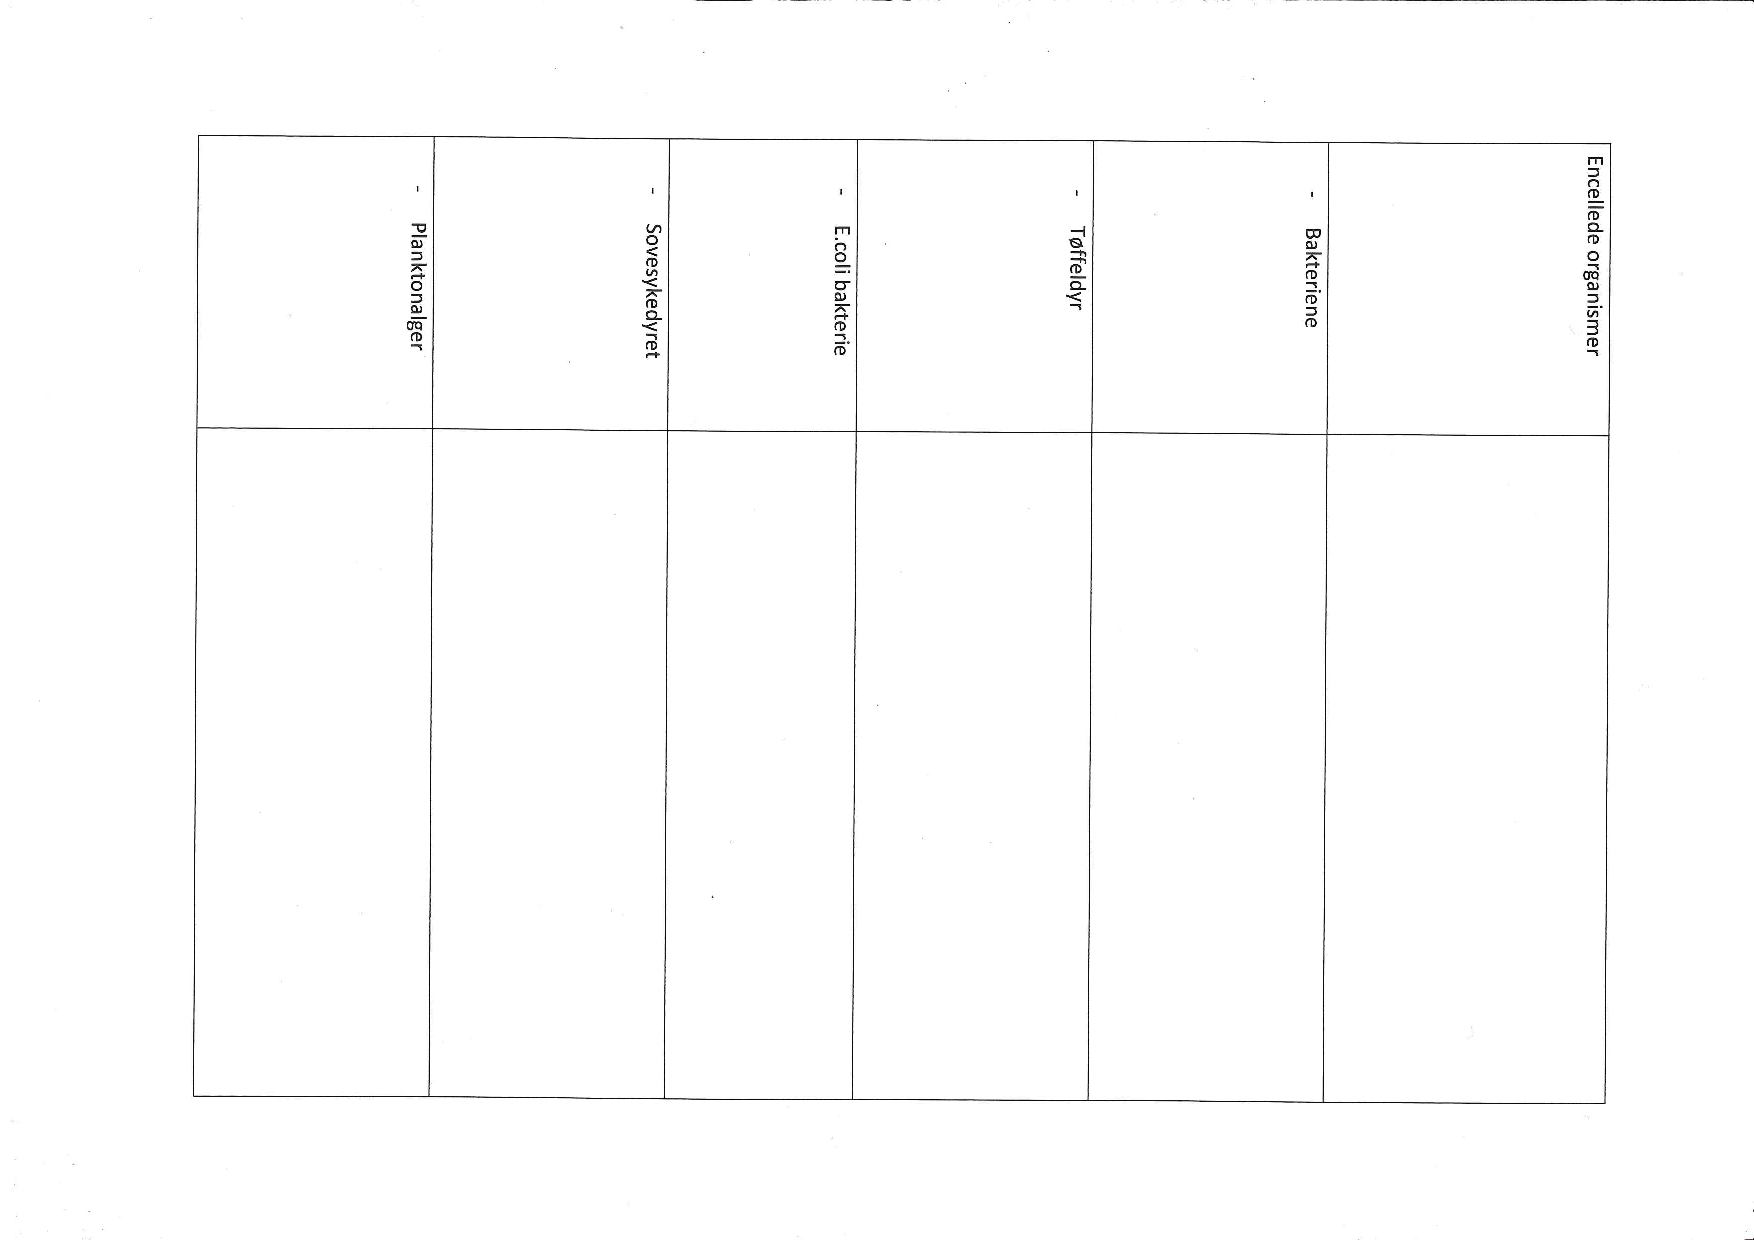
\includepdf[scale = 0.90,angle=90]{../figures/tokolonnenotat_side2.pdf}
%\restoregeometry
\end{document}
